% !TEX root = diplomarbeit.tex
\chapter{Sensoren}
\renewcommand{\kapitelautor}{Autor: Lucas Ullrich}

%%%%%%%%%%%%%%%%%%%%%%%%%%%%%%%%%%%%%%%%%%%%%%%%%%%%%%%%%%%%%%%%%%%%%%%%%%%%%%%
\section{PIXY CMUcam5}
Bei der PIXY CMUcam5 handelt es sich um ein Open Source Kameramodul, welches über eine Objekterkennung verfügt.
Mit diesem ist es möglich sogenannte Colorcodes oder einfache Objekte zu erkennen.

\begin{figure}[H]
  \begin{centering}
    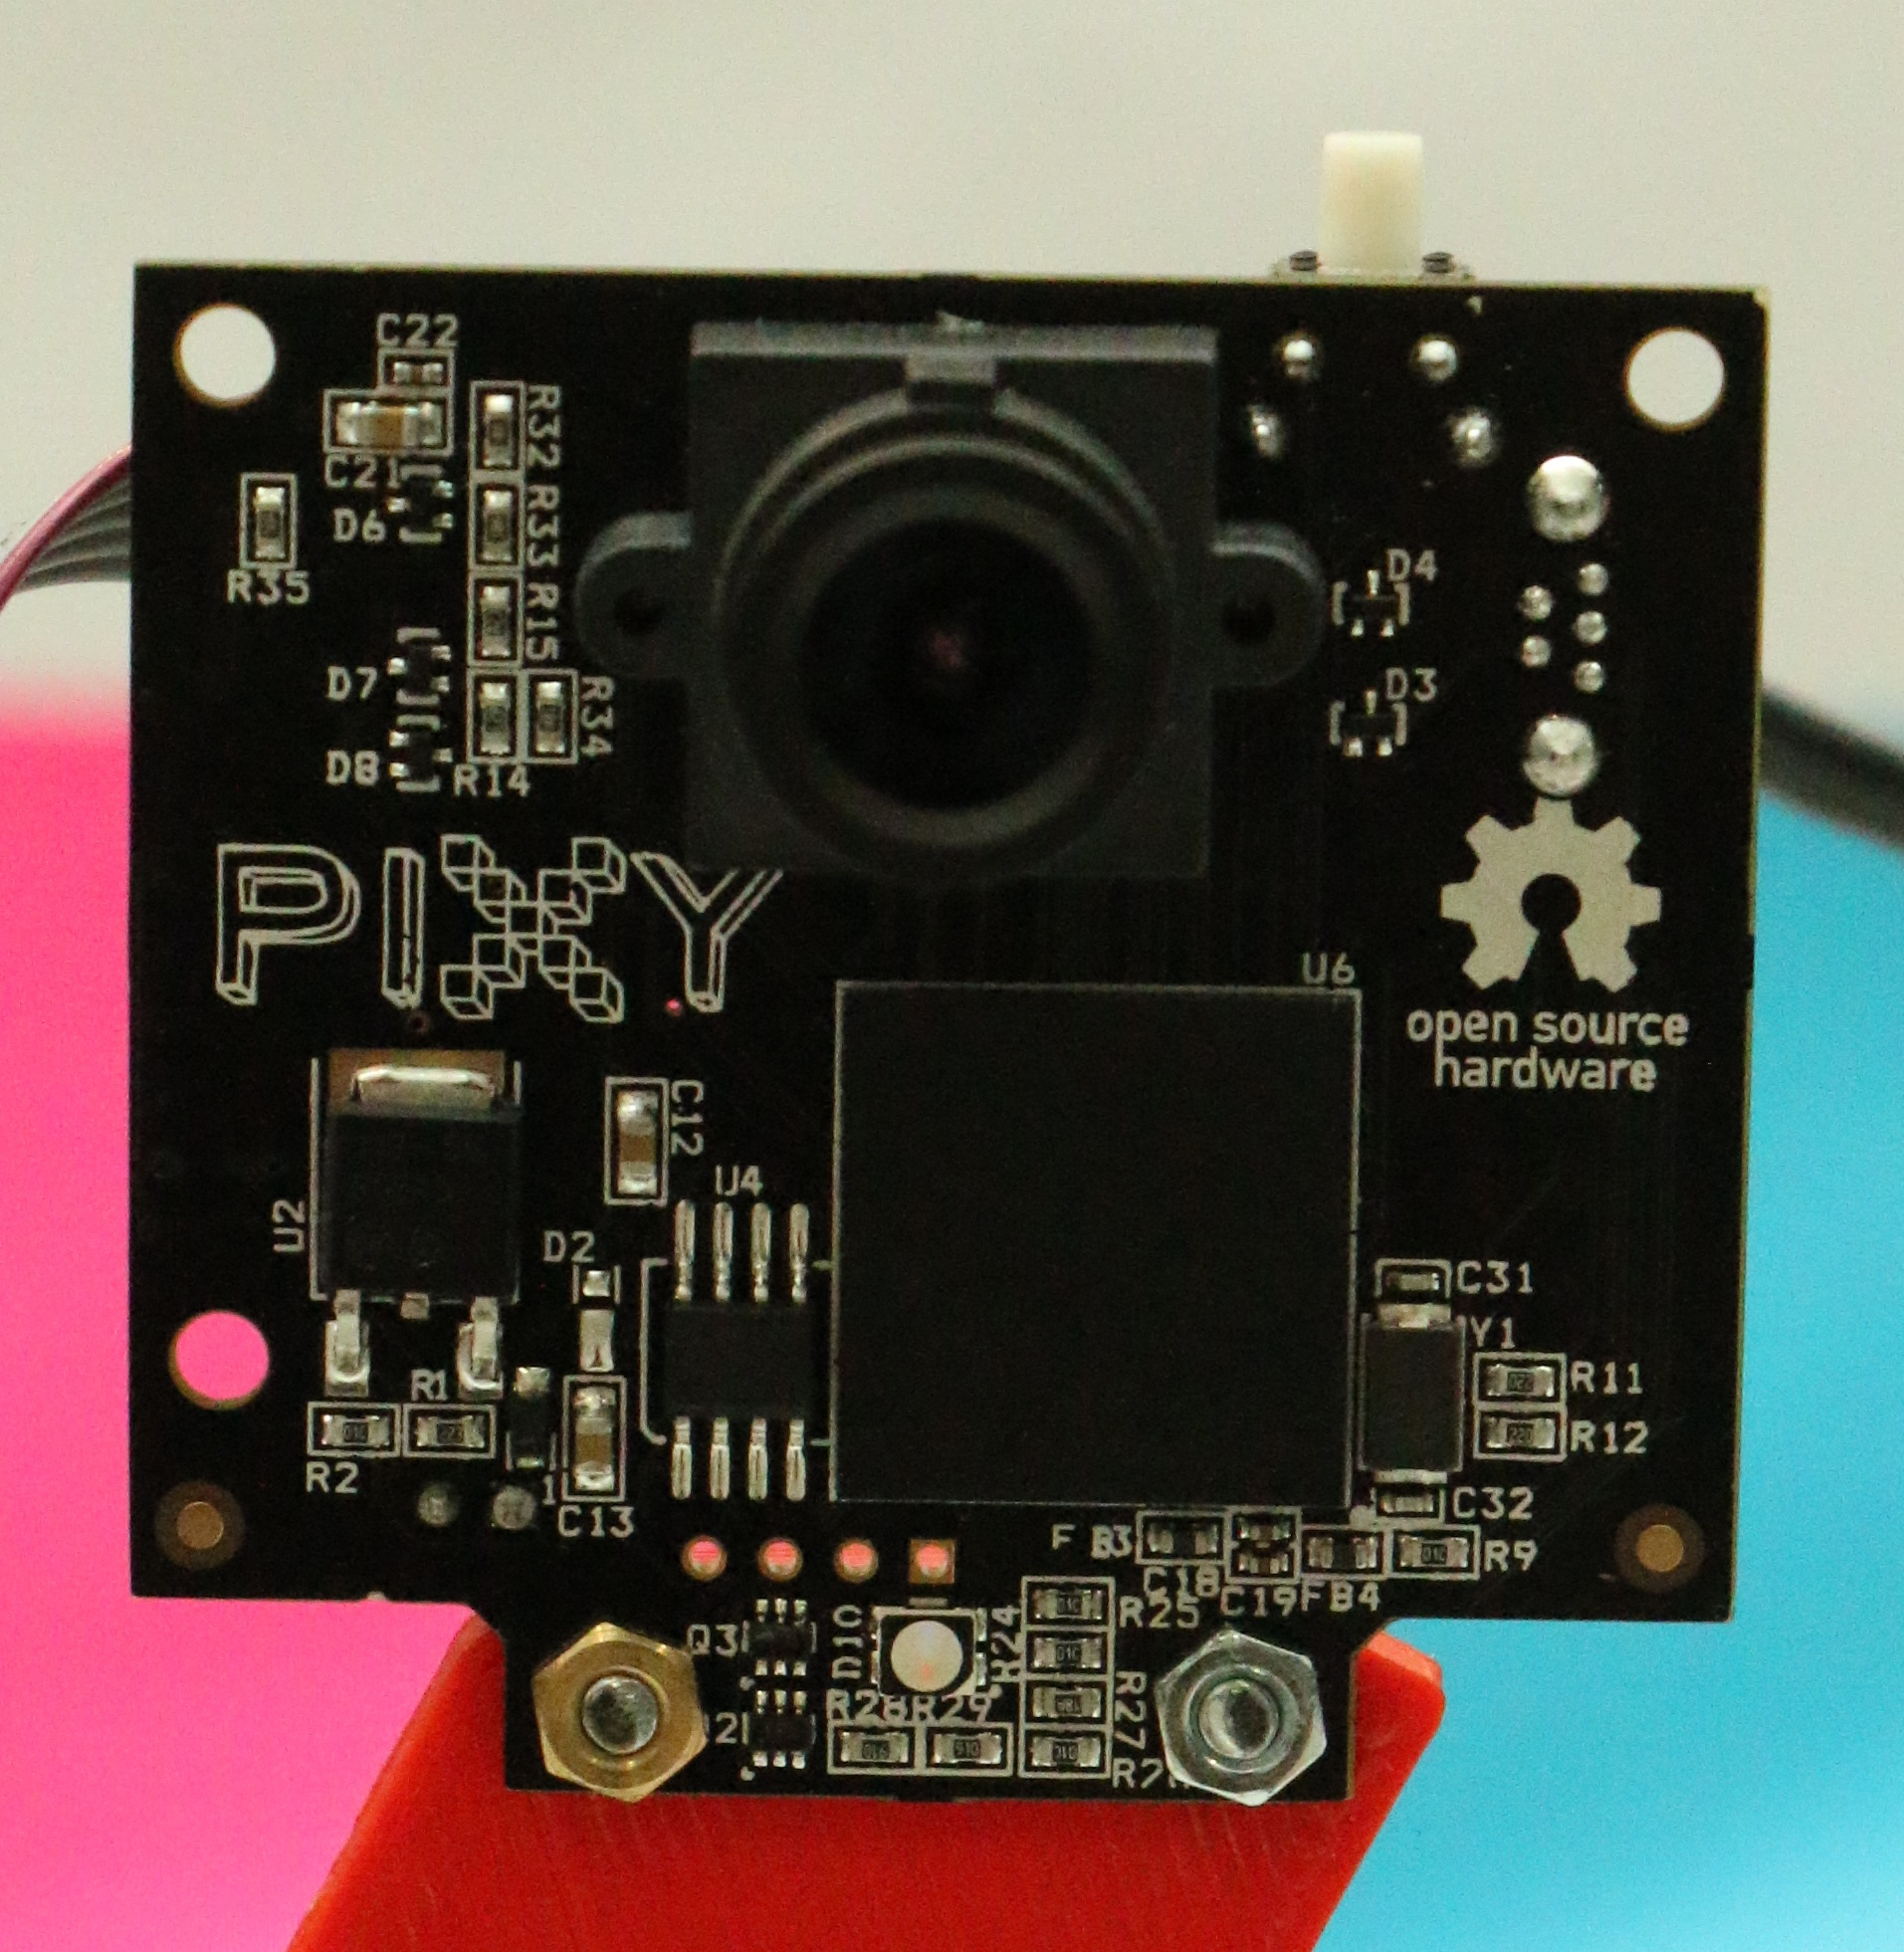
\includegraphics[width = 0.4\textwidth]{Bilder/Pixy_CMUcam5}
  \par\end{centering}
  \caption{PIXY CMUcam5}
  \label{PIXY}
\end{figure}

\begin{figure}[H]
  \begin{centering}
    \subfigure[Colorcode]{
\includegraphics[width = 0.4\textwidth]{Bilder/Colorcode}}
    \subfigure[Objekt]{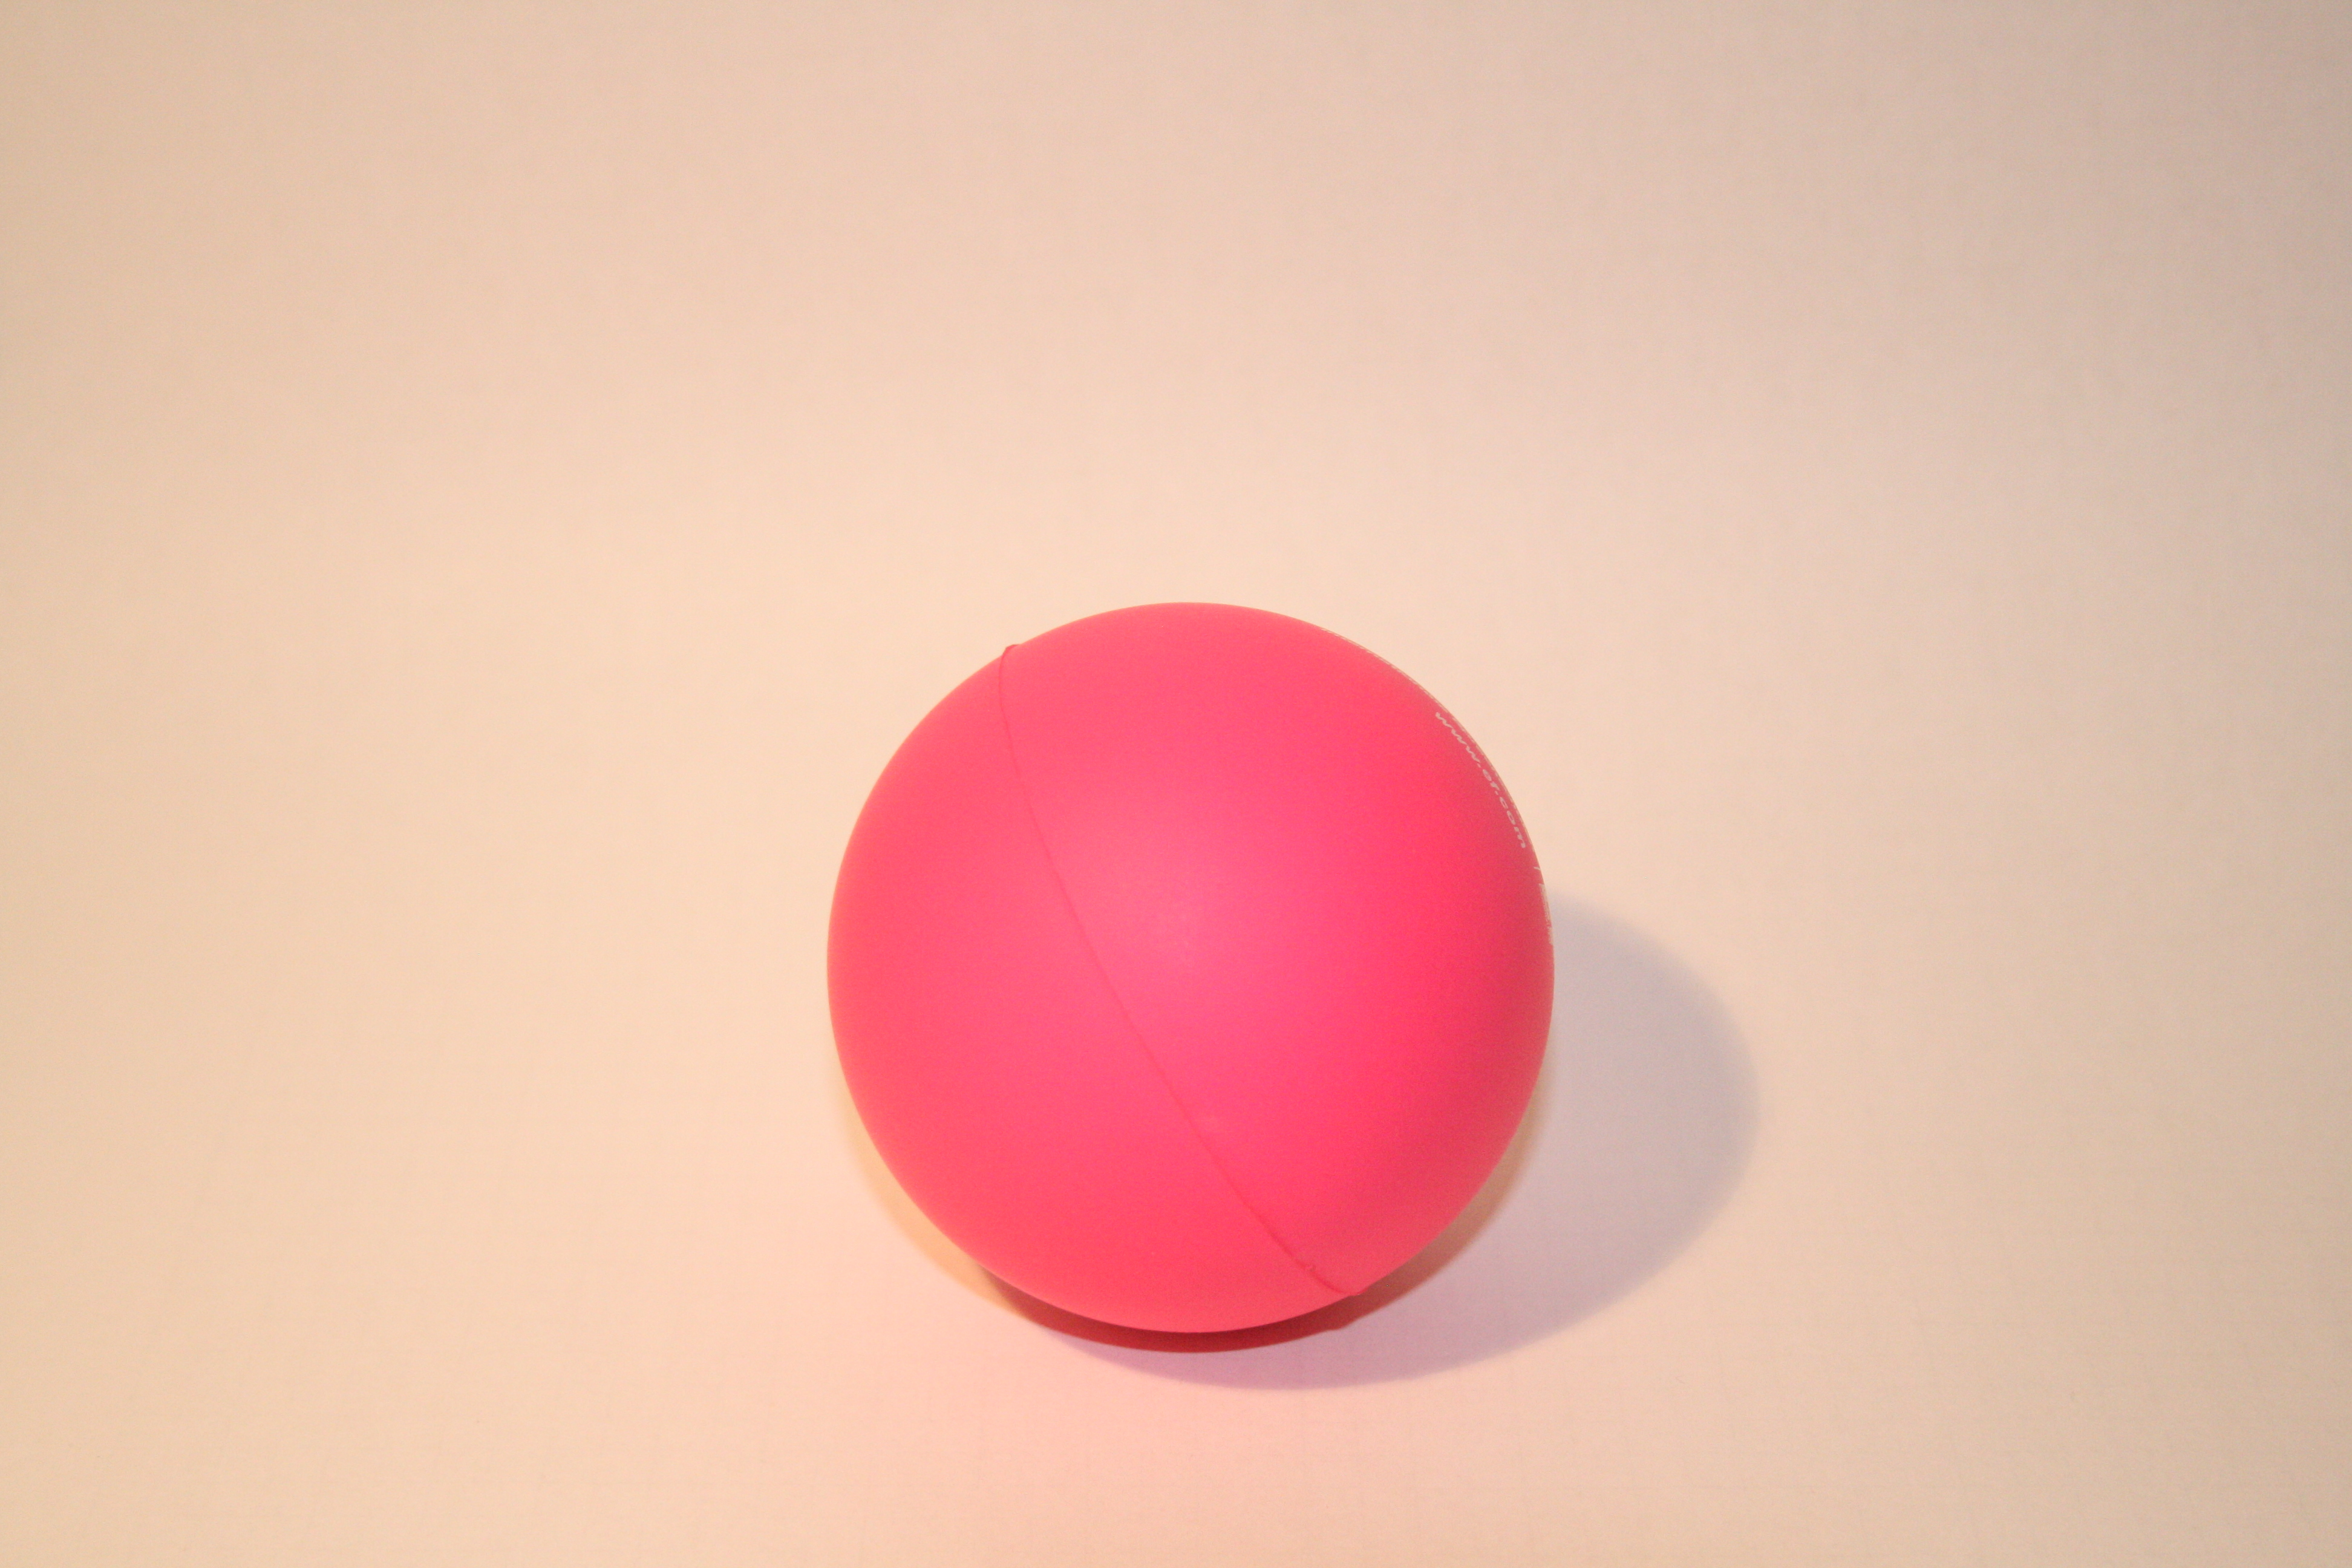
\includegraphics[width = 0.4\textwidth]{Bilder/Objekt}}
  \par\end{centering}
  \caption{Erkennbare Objekttypen}
  \label{PIXY_Objekte}
\end{figure}

\needspace{2cm}
  \subsection{Technische Planung}
    \subsubsection{Mögliche Verfahren zur Positionserkennung}
    Hier muss grundsätzlich zwischen zwei Messmethoden unterschieden werden:
    \begin{itemize}
      \item \textbf{Absolute Positionsmessung}\\
      Hier wird die Position von einem gleichbleibenden Punkt aus gemessen. Dabei ist ein konstanter Referenzpunkt wichtig.
      Verändert sich dieser oder kann die Distanz nicht genau gemessen werden ist die Messung unbrauchbar.

      Für eine absolute Positionsmessung bieten sich diverse Triangulationsverfahren an,
      diese sind ausgesprochen rechenaufwändig und benötigen meist eine sehr genaue Laufzeitmessung.
      Für die Triangulation können die unterschiedlichsten Signale verwendet werden, am gängigsten sind jedoch jene die mit elektromagnetischen Wellen arbeiten,
      \zB WLAN, Bluetooth. Dies bedeutet, dass sich die Signale mit Lichtgeschwindigkeit ausbreiten.

      Bei einer Messung derart schneller Signale muss ein hoher Aufwand betrieben werden um eine Messgenauigkeit von einigen cm zu erzielen.
      Eine weitere Herausforderung sind Mauern \bzw Hindernisse. Hier muss ständig berücksichtigt werden wo ein Objekt steht und ob der geplante Weg überhaupt frei ist.
      \item \textbf{Relative Positionsmessung}\\
      Hier wird die Position von einem wechselnden Punkt aus gemessen. Um hier eine Positionierung im Raum ermöglichen zu können,
      ist es erforderlich immer zu einem bestimmten Punkt zu messen. Ein Wechsel dieses Punktes ist jedoch möglich,
      deshalb muss auch die Position der Punkte im Raum bekannt sein. Ist die Zielposition im Raum bekannt kann zu dieser hin navigiert werden.
      Auch hier muss wie bei einer absoluten Positionsmessung auf Hindernisse geachtet werden.

      Die zweite Alternative ist, dass eine bestimmte Route bekannt ist und sich das zu positionierende Objekt nur in einem bestimmten Bereich um diese Route bewegt.
      Wird bei der Positionierung der Route bereits auf Hindernisse geachtet müssen diese im Anschluss nicht mehr zwingend beachtet werden.
    \end{itemize}

  \subsection{Umsetzung}
  Durch die PIXY CMUcam5 lässt sich eine relative Positionsmessung vergleichsweise einfach verwirklichen.
  Werden ein oder mehrere Objekte erkannt wird eine bestimmte Nummer (abhängig von der Farbe) sowie die Position am Bild und die Objektgröße übermittelt.
  Die Kamera arbeitet dabei mit einer Bildwiederholrate von 50 Hz, es ist also alle 20 ms eine Auswertung möglich.

  Die Kamera wird auf dem Hexacopter befestigt, mehrere Farbcodes kennzeichnen den Weg zu einem Tisch.
  Um an dieser Stelle eine Navigation zu erreichen wird der Hexacopter so gesteuert, dass er, abhängig von der Route,
  immer einen bestimmten Farbcode betrachtet, ist er über diesem sucht er den nächsten.

    \subsubsection{SPI Schnittstelle}
    Als Schnittstelle für die Kommunikation mit der Kamera wird eine SPI-Schnittstelle verwendet.
    Die Kamera selbst unterstützt unter anderem die seriellen Schnittstellen UART, I2C und SPI.
    Außerdem werden noch ein analoger und digitaler Output unterstütz, diese sind jedoch vergleichsweise beschränkt,
    da keine näheren Informationen zu dem Objekt übermittelt werden können sondern nur die Position \bzw ob überhaupt ein Objekt erkannt wurde.

    Die SPI-Schnittstelle ist bei der Kamera besonders ausfallsicher. Hier wird ein Synchronisationsbyte gefordert, wird dieses nicht erkannt,
    \zB aufgrund eines Fehlers in der Datenübertragung, schickt die Kamera keine Daten.

    \paragraph{Überprüfen der SPI-Schnittstelle}
    Um zu überprüfen ob die SPI-Schnittstelle auch korrekt arbeitet wird bei der ersten Inbetriebnahme der Output überprüft.
    Hierzu wird der Zustand der 3 Leitungen mit einem Oszilloskop betrachtet.
    \begin{itemize}
      \item \textcolor{blue}{Taktleitung}
      \item \textcolor{red}{Dateneingang (PIC)}
      \item \textcolor{green}{Datenausgang (PIC)}
    \end{itemize}

    \begin{figure}[tbh]
      \begin{centering}
        \subfigure[Großer Zeitbereich]{\includegraphics[width = 0.49\textwidth]{Bilder/SPI_gross}}
        \subfigure[Kleiner Zeitbereich]{\includegraphics[width = 0.49\textwidth]{Bilder/SPI_klein}}
      \par\end{centering}
      \caption{Ausgang der SPI Schnittstelle}
      \label{SPI-Ausgang}
    \end{figure}

    Der Wert mit dem diese Überprüfung durchgeführt wird sollte möglichst variabel sein, hier wird 0xAA (1010 1010) verwendet.
    Wird dieser Wert nicht variabel angenommen kann es dazu kommen, dass fälschlicher Weise angenommen wird, dass die Übertragung korrekt ist.
    Der Dateneingang des PIC, respektive der Ausgang der Kamera, zeigt eine deutliche Störung durch die Taktleitung an.

    \subsubsection{Erkennen und Auswerten eines Bildes}
    Die Kamera schickt der Reihe nach die einzelnen Daten eines Objekts. Darunter ist auch eine Startbedingung welche ein neues Bild markiert.
    Mit den diversen Informationen zum Objekt ergeben sich folgende Daten:
    \begin{itemize}
      \item Neues Bild 0xAA55
      \item Objekt 0xAA55 oder Farbcode 0xAA56
      \item Checksum
      \item Objektnummer
      \item X-Position
      \item Y-Position
      \item Breite
      \item Höhe
      \item Drehwinkel, nur bei Farbcodes
    \end{itemize}
    Dabei ist die Objektnummer von den im Objekt oder Farbcode vorkommenden Farben abhängig, zusätzlich ist zu beachten, dass sie oktal dargestellt wird.
    Ein übermittelter Wert von dezimal 10, also oktal 12, bedeutet, dass die Farben 1 und 2 erkannt wurden.

    Will man nun ein neues Bild finden muss man so lange nach 0xAA55 suchen bis man diese Daten gesendet bekommt.
    Anschließend gilt es noch festzustellen ob man einen Farbcode oder ein Objekt betrachtet,
    es muss also direkt darauf 0xAA56 oder nochmals 0xAA55 erkannt werden. Ist dies nicht der Fall, wurde kein neues Bild erkannt und man betrachtet ein normales Objekt.

    Betrachtet man nun die bis zum Erkennen eines neuen Bildes gesendeten Daten als gegenstandslos ergibt sich eine vergleichsweise einfache Schleife um ein Bild zu erkennen.

    \lstset{language = c}
    \begin{lstlisting}
while(frame == 0) {
  w = ExchangeSpiWord(PIXY_SYNC, DUMMY);
  if(lw == PIXY_FRAME_OBJ && w == PIXY_FRAME_OBJ) {
    frame = 1;
    obj_type = 0;
    a_color[c_obj].type = PIXY_FRAME_OBJ;
  } else if(lw == PIXY_FRAME_OBJ && w == PIXY_COLORCODE) {
    frame = 1;
    obj_type = 1;
    a_color[c_obj].type = PIXY_COLORCODE;
  } else if(w == 0 && lw == 0){
    frame = 0;
  }
  lw = w;
  c++;
  if(c > 254) {
    return 0;	//****Error, end of function
  }
}
    \end{lstlisting}
    Um nicht ewig in dieser Schleife fest zu hängen, wenn kein Bild erkannt wird und einen Fehler auslösen zu können wird die gesamte Funktion der Bildauswertung
    nach 255 Versuchen verlassen.

    Die weiteren Werte eines Objekts werden der Reihe nach in einer \gls{Struktur} abgespeichert, hier ist nichts Besonderes mehr zu beachten.

  \subsection{Herausforderungen und Lösungen}
  Besonders das Beispielprogramm\cite{PIXY_Porting_Examplecode} für eine Bildauswertung stellte einige Herausforderungen dar. Hier sind unterschiedliche Codeschnippsel in einem
  großen Beispiel zusammengefasst. Das ist besonders bei durch die ähnlichen Funktionen des Codes schwer auseinander zu halten. So steht eine Funktion für die Erkennung eines
  neuen Bildes, diese zählt aber nur Bilder pro Sekunde, eine andere ist dann für die gesamte Auswertung und sucht dafür erneut nach einem Bild.

  Diese Zusammenhänge konnten durch einige Überlegungen erkannt werden und darauffolgend die eigene Firmware geschrieben werden.

  Ein weiteres Problem stellt die Empfindlichkeit der Kamera bei wechselnden Lichtverhältnissen dar. Da diese über die Farbsignatur eines Objektes arbeitet werden bereits
  sehr kleine Differenzen unterschieden um verschiedene Objekte erkennen zu können \bzw keine Störungen durch den Hintergrund zu erhalten. Dies wird jedoch ebenso in der
  anderen Richtung zu einem Problem. Wechselt das Licht ein wenig kann ein Farbcode oft nicht mehr zuverlässig erkannt werden und die Kamera muss über einen Computer nachkalibriert
  werden. Eine mögliche Lösung ist das konstante Beleuchten der Farbcodes mit einer sehr bestimmten Leuchtstärke, hier kann es leicht zu Überbelichtungen kommen, besonders bei
  dunklen Verhältnissen, als auch die Umrüstung auf einen \gls{Infrarot}-Kit. Bei einem Infrarot-Kit fällt jedoch die Individualität jedes einzelnen Markers weg.

%%%%%%%%%%%%%%%%%%%%%%%%%%%%%%%%%%%%%%%%%%%%%%%%%%%%%%%%%%%%%%%%%%%%%%%%%%%%%%%
\section{Ultraschallsensor HC-SR04}
Der Ultraschallsensor HC-SR04 ist ein für Arduino entwickeltes Modul um Abstände zu messen. Die Messung geschieht durch das Aussenden von Ultraschallimpulsen,
die Messgröße wird dabei als laufzeitabhängiger Impuls retourniert.

\begin{figure}[tbh]
  \begin{centering}
    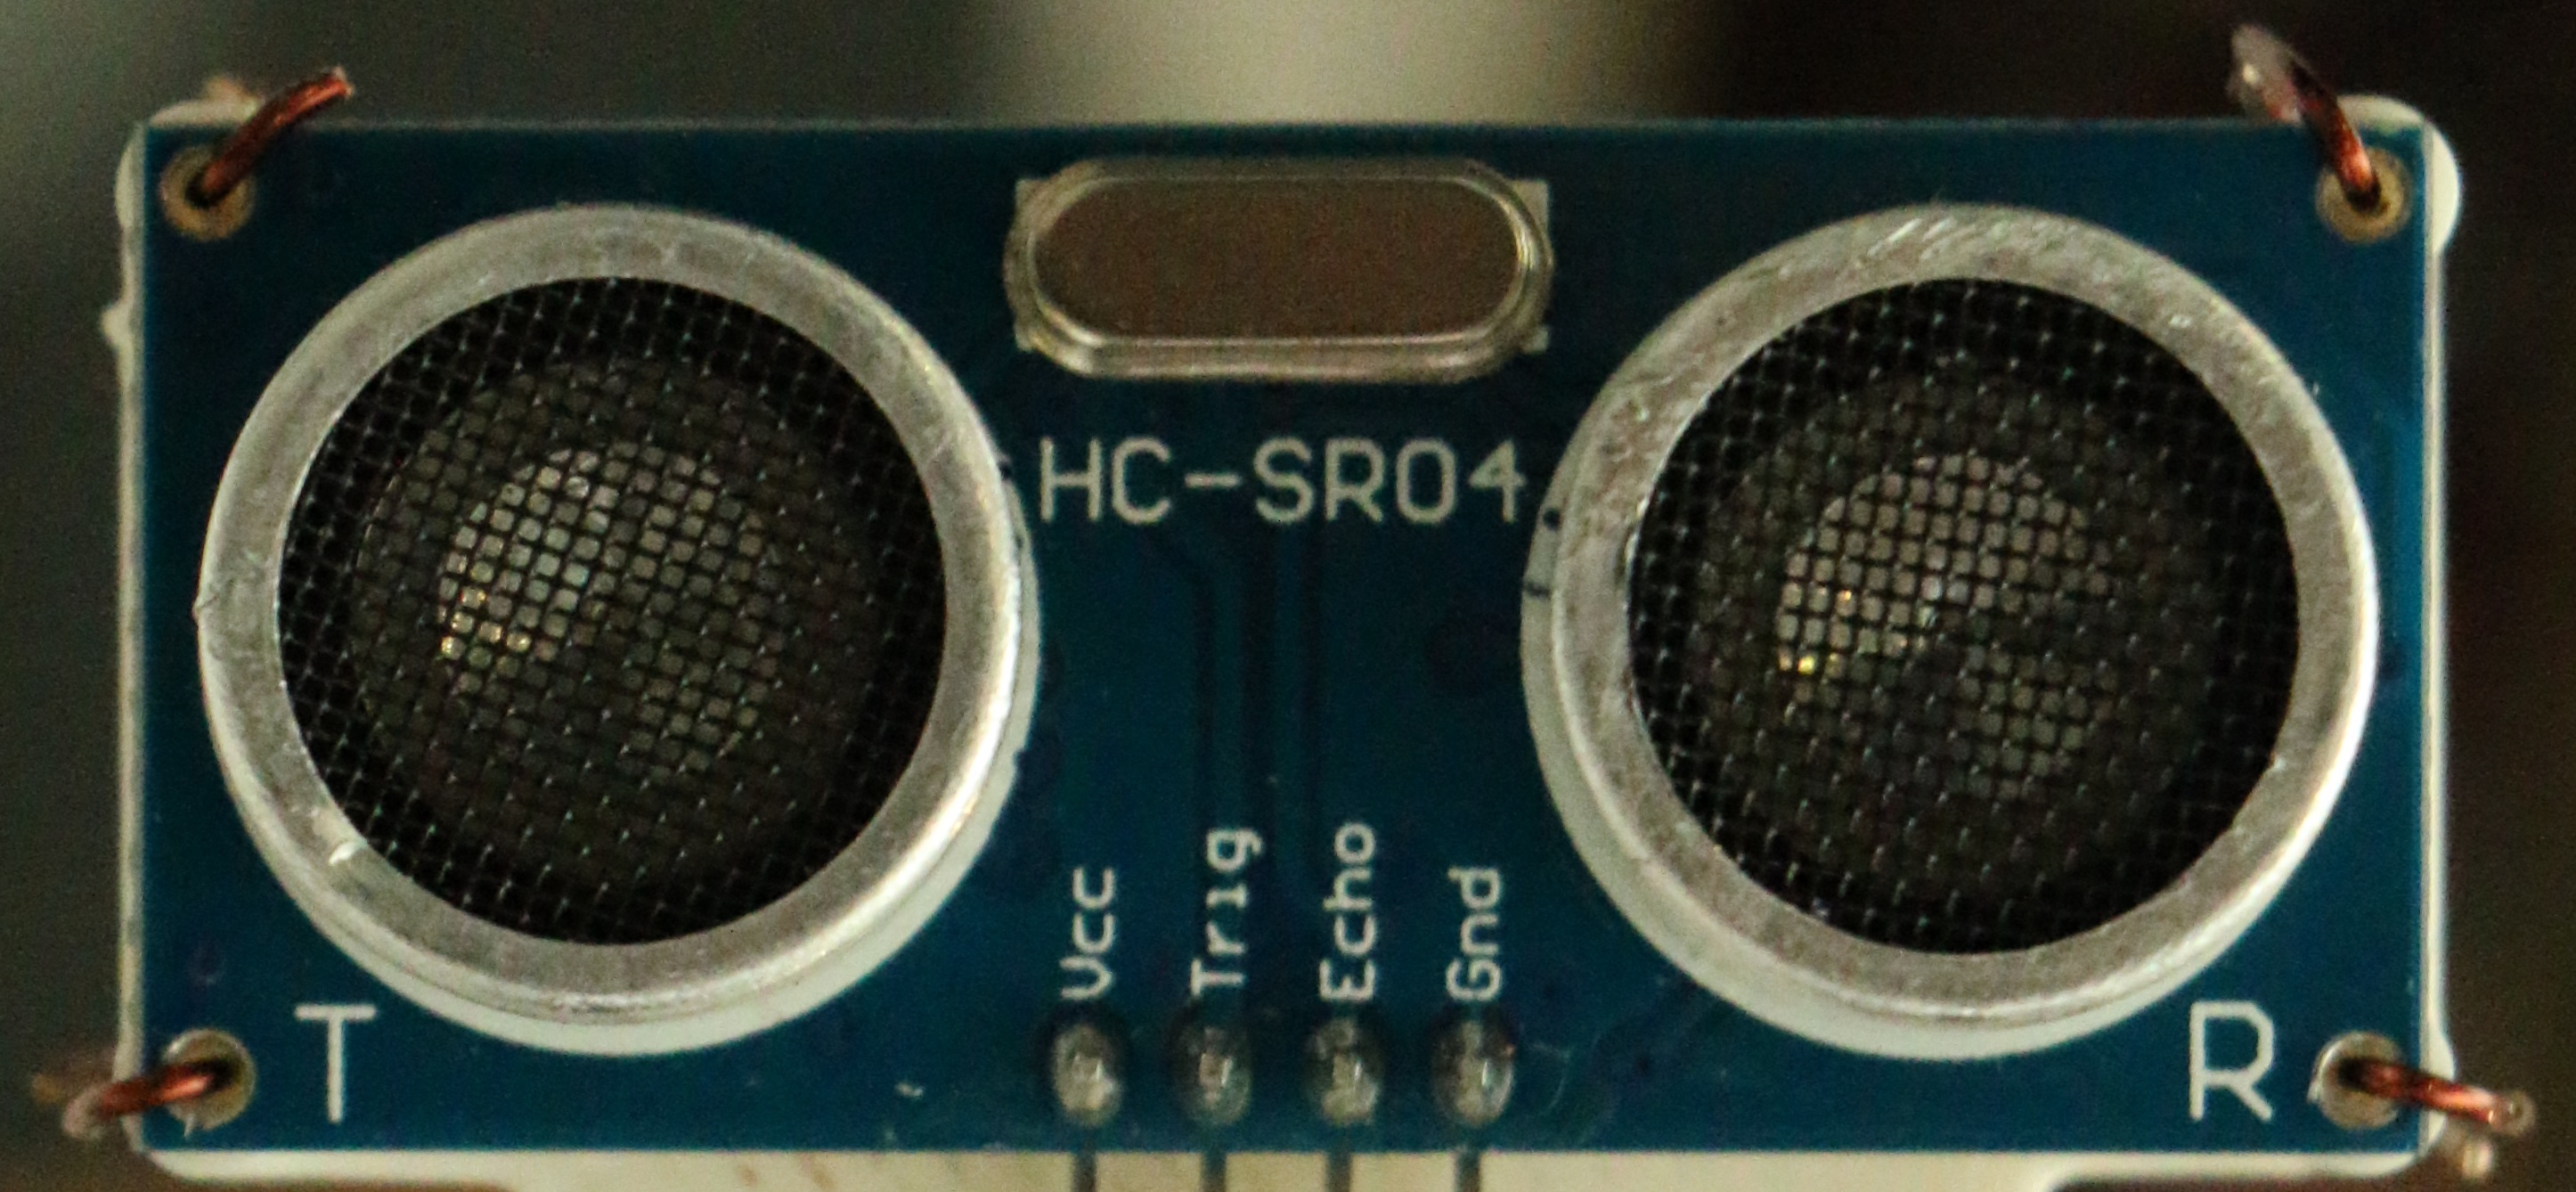
\includegraphics[width = 0.5\textwidth]{Bilder/Ultraschallsensor}
  \par\end{centering}
  \caption{Ultraschallsensor HC-SR04}
  \label{Ultraschallsensor}
\end{figure}

  \subsection{Technische Planung}
  Für die Steuerung des Hexacopter ist es notwendig die aktuelle Flughöhe zu wissen.
  Es ist mit einer bekannten Objektgröße und den von der Kamera vorliegenden Daten zwar möglich die aktuelle Flughöhe rechnerisch zu bestimmen,
  jedoch gestaltet sich dies sehr rechenaufwändig. Um die Höhe möglichst einfach messen zu können bietet sich daher eine vergleichsweise langsame Messung,
  wie jene mit einem Ultraschallsignal an.
  Bei einer Schallgeschwindigkeit von $\SI{343}{\meter\per\second}$ entstehen bei einer zu messenden Distanz von $\SI{2}{\meter}$,
  Laufzeiten des Ultraschallsignals von \ca $\SI{12}{\milli\second}$ (Distanz mal 2 da das Signal wieder zurückkehren muss).

  \subsection{Umsetzung}
  Abhängig von der mit dem Mikroprozessor ermittelten Laufzeit $time\_height$ lässt sich jederzeit die aktuelle Flughöhe bestimmen.
  \[
  s(time\_height) = \frac{v \cdot t}{2} = \frac{\SI{343}{\meter\per\second} \cdot time\_height}{2}
  \]
  Die Höhe wird dabei in der main-Routine durch den Aufruf folgender Funktionen regelmäßig bestimmt:
  \lstset{language = c}
  \begin{lstlisting}
void StartHeightMeasure(void) {
  TMR5L = 0;
  TMR5H = 0;
  Trigger = 0;
}

void ReadHeight(void) {
  while(TMR5GIF == 0);
  TMR5GIF = 0;
  time_height = 0;
  time_height = TMR5H;
  time_height <<= 8;
  time_height |= TMR5L;
  TMR5L = 0;
  TMR5H = 0;
  a_frame[0].height = time_height;
  a_frame_dif[0].dif_height = a_frame[1].height - a_frame[0].height;
  Trigger = 1;
}
  \end{lstlisting}

  In der ersten Funktion wird die Messung gestartet. Dazu wird ein Trigger-Signal an den Ultraschallsensor gesendet, dieser reagiert auf eine fallende Flanke.
  Zuvor wird darauf geachtet, dass die Register in denen die Zeit zurückgegeben wird auch wirklich leer (= 0) sind.
  In der zweiten Funktion folgt das Auslesen der vorhandenen Daten. Dazu werden die zwei 8-Bit Register in der 16-Bit Variable $time\_height$ abgespeichert.
  Zusätzlich wird die gemessene Höhe für die Auswertung in der $a\_frame[0].height$ Variable abgespeichert und die Differenz zur vorhergehenden Messung ermittelt.

  Auf eine Berechnung der genauen Höhe in m wird zu Gunsten der Verarbeitungszeit verzichtet, auf die spätere Auswertung der Flugdaten hat dies keinen Einfluss.

  \subsection{Herausforderungen und Lösungen}
  \textcolor{red}{to be continued after realtime measurements}

\chapter{Aktoren}
\renewcommand{\kapitelautor}{Autor: Christina Bornberg, Lucas Ullrich}

%%%%%%%%%%%%%%%%%%%%%%%%%%%%%%%%%%%%%%%%%%%%%%%%%%%%%%%%%%%%%%%%%%%%%%%%%%%%%%%
\section{Multicopter Chrisy}
  Multicopter gehören zu der Luftfahrzeuggattung Hubschrauber. Sie starten senkrecht und können durch den Antrieb der Rotoren Neigung erzeugen. Durch diese Neigung kann der Hexacopter nach vorne, zurück, nach links und nach rechts fliegen. Durch die Rotoren, bei denen sich abwechselnd einer nach links und einer nach rechts dreht, kann sich der Hexacopter zusätzlich um seine Hochachse drehen.

  \subsection{Funktion Chrisy}
  Ein Multicopter besteht im Normalfall aus folgenden Komponenten:
  Dem Empfängermodul, dem DJI NAZA-M Flightcontroller sowie der Multicopterhardware (Rotoren, Motoren, Gestell und Leistungselektronik). Der Empfänger des Multicopters kann von einem Sender Steuersignale empfangen und aufgrund der empfangenen Steuersignale Soll-Werte für die Motoren berechnen, um den Multicopter auf die entsprechende Höhe bzw. entsprechende Geschwindigkeit in x, y oder z Richtung zu bringen.

  % BILD Funktion Blockschaltbild (Dokument) %

  \subsection{Erweiterte Funktion Chrisy}
  Im Rahmen dieser Diplomarbeit wurden die üblicherweise verwendeten Teile um vier weitere Komponenten erweitert, um einen automatischen Flug zu gewährleisten: Pixycam, Ultraschallsensor, WLAN Modul und ein Mikrocontroller. Pixycam und Ultraschallsensor sind dafür verantwortlich, die Daten für die Berechnung der augenblicklichen Position des zu bestimmen. Im Mikrocontroller läuft ein Algorithmus, der aus diesen empfangen Daten die Position überprüft. Wenn der Wert vom optimalen Bereich abweicht, werden die Steuersignale abgeändert. Durch das Wlan-Modul bekommt der Mikrocontroller die Information, durch wie viele Marker der Weg definiert ist und welcher Farbcode der letzte ist, auf dem die Landung erfolgt.

  % BILD %

  \subsection{Multicopter Arten Chrisy}
  Es gibt verschiedene Arten von Multicoptern. 
  Je nachdem wie viele Rotoren in einer Ebene liegen, setzt sich der Name zusammen.
  Die bekannteste Art ist der Quadrocopter, welcher 4 Rotoren besitzt. Weiters gibt es Hexacopter mit 6 und Octocopter mit 8 Rotoren. \cite{GrundlagenMulticopter}

  Der Flightcontroller DJI Naza-M lite unterstützt verschiedene Konfigurationsarten von Quadrocoptern und Hexacoptern. Hierzu zählen + und x Konfiguration für den Quadrocopter. Beim Hexacopter gibt es die Varianten +, x, reverse Y und Y. Diese werden im nächsten Abschnitt genauer beschrieben. \cite{NAZA_Konfig}

  \subsection{Konfiguration Chrisy}
  Grundsätzlich gibt es 2 Arten einen Multicopter zu Konfigurieren. \cite{GrundlagenMulticopter}
  Einerseits die +- beziehungsweise I-Konfiguration, andererseits die x- beziehungsweise H-Konfiguration. Weiters gibt es die weniger verbreitete Y-Konfiguration. Dabei geht es um die Ausrichtung und die damit verbundene Fluglage. 

  Für diese Diplomarbeit wurde die + Konfiguration für Hexacopter gewählt.

  Wie auf folgender Grafik ersichtlich ist, gibt es nach links und nach rechts drehende Rotoren. Die rot gekennzeichneten Arme geben an, wo die Vorderseite des Multicopters ist. Bei der Y-Konfiguration sind die blau Makierten Propeller oben, die Roten unten.

  % BILD mit 4, 6, 8 in + bzw x %

  \subsection{Mögliche Anwendungsgebiete Chrisy}
  Multicopter finden in vielen Bereichen Anwendung. \cite{copterAnwendung}
  \begin{itemize}
    \item Fotographie und Videos / Filmindustrie / Anfertigen von hoch aufgelösten Luftbildkarten
    \item Multicopter als Hobby / Kunstflug
    \item Lagerhallen und Logistik / Bestands- und Inventaraufnahmen im Straßenbau
    \item Forschung / Schwarmverhalten
    \item Multicopter als Lebensretter / Rettungseinsätze / Katastrophenschutz
    \item Unterstützung der Polizei / große Menschenmengen überwachen
    \item Unbemannter Aufklärer bei Spezialeinheiten
    \item Kontrolle, Inspektion und Dokumentation von Brücken, Gebäuden, Gräben
    \item Militärische Anwendung: Spionagedrohne zur Aufklärung, Kampfdrohne zur Zerstörung, Rettungungsdrohne für Hilfsaktionen
  \end{itemize}  
  

\section{Rotoren}

  \subsection{Technische Planung Lucas}

  Der Hexacopter selbst vefügt über 6 Rotoren. Diese werden für die unterschiedlichen Flugrichtungen von dem Flightcontroller angesteuert.
  Der Flightcontroller liest die Daten an den einzelnen Steuerpins als Servo-Impulse ein. Die Daten werden dabei in einer Periode von $\SI{20}{\milli\second}$ gesendet.
  Die Information selbst liegt in den ersten $\SI{2}{\milli\second}$. Für den Impuls beträgt die Mittelstellung $\SI{1.5}{\milli\second}$, das Minimum $\SI{1}{\milli\second}$
  und das Maximum $\SI{2}{\milli\second}$. Das Signal folgt somit den Konventionen eines Servo-Impulses.

  \textcolor{red}{OSZIBILD: min, max Impuls}


    \subsubsection{Steuerungsarten Chrisy}
    Der Flightcontroller DJI NAZA-M lite wird über die Befehle Aileron, Elevator, Rudder und Throttle gesteuert. Zusätzlich gibt es den 2/3-position mode channel, der für das Umschalten mehrerer Modei zuständig ist. Handelsübliche Fernbedienungen verfügen über die selben Steuerbefehle. \cite{GrundlagenMulticopter}

      \begin{itemize}
        \item \textbf{A: Aileron} auch Rollen (engl. roll) genannt, ist für die Bewegung nach Links und Rechts zuständig.
        Um diese auszuführen, werden bei der Beschleunigung nach links, die rechten Propeller stärker betrieben, umgekehrt drehen sich die auf der linken Seite befindlichen Propeller beim Flug nach rechts schneller. Durch die entstehende Neigung, fliegt der Hexacopter in die gewünschte Richtung.
        \item \textbf{E: Elevator} auch Nicken (engl. pitch) genannt, ist für die Vorwärts- und Rückwärtsbewegung zuständig.
        Beim nach vorne und nach hinten fliegen, werden ebenfalls die rotoren schneller betrieben, die auf der jeweils gegenüberliegenden Seite liegen. 
        \item \textbf{R: Rudder} auch Gieren (engl. yaw) genannt, ist für die Rotation an der Hochachse zuständig.
        Um den Hexacopter um seine eigene Hochachse rotieren zu lassen, werden für eine Rotation nach rechts, die rechts-drehenden Rotoren schneller betrieben, bei der Rotation nach Links, die links-drehenden.
        \item \textbf{T: Throttle} reguliert die Höhe.
        Bei gleichmäßiger Ansteuerung der 6 Rotoren, kann man je nach Drehgeschwindigkeit die Höhe verändern. Der Hexacopter fliegt bei stärkerer Beschleunigung nach oben, ansonsten sinkt er. Dies wird auch als Uplift and Downfall bezeichnet.
        \item \textbf{U: 2/3-position switch channel} ist zum Umschalten von zwei oder drei Steuermodi zuständig. Im Fall unserer Diplomarbeit wird zwischen autonomem und manuellem Flug gewechselt. \cite{positionswitch}
      \end{itemize}

    % BILD Fernsteuerung%

  \subsection{Umsetzung}
  Um den Hexacopter steuern zu können müssen die einzelnen Impulse von dem Mikrocontroller imitiert werden.

  \subsection{Herausforderungen und Lösungen}
